\documentclass[border=4pt]{standalone}
\usepackage{amsmath,amssymb,amsfonts}
\usepackage{xcolor,colortbl,array,booktabs,multirow}
\usepackage{tikz}
\usetikzlibrary{arrows, automata, backgrounds, calendar, chains, decorations,
    matrix, mindmap, patterns, petri, positioning, shadows, shapes.geometric,
    trees, shapes, decorations.pathreplacing, calc, tikzmark, arrows.meta}
\newcommand{\st}{\text{ s.t. }}
\newcommand{\x}{\mathbf{x}}
\renewcommand{\b}{\mathbf{b}}
\newcommand{\A}{\mathbf{A}}
\newcommand{\R}{\mathbb{R}}
\newcommand{\RR}{\mathbb{R}}
\newcommand{\Z}{\mathbb{Z}}
\newcommand{\ZZ}{\mathbb{Z}}
\begin{document}
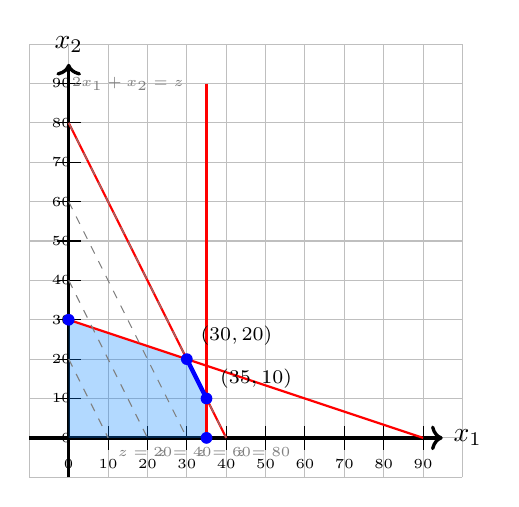
\begin{tikzpicture}[scale=0.05]
    % Grid and axes
    \draw[gray!50, thin, step=10] (-10,-10) grid (100,100);
    \draw[very thick,->] (-10,0) -- (95,0) node[right] {$x_1$};
    \draw[very thick,->] (0,-10) -- (0,95) node[above] {$x_2$};

    \foreach \x in {0,10,...,90} \draw (\x,3) -- (\x,-3) node[below] {\tiny\x};
    \foreach \y in {0,10,...,90} \draw (-3,\y) -- (3,\y) node[left] {\tiny\y};

    % Feasible region
    \fill[blue!50!cyan,opacity=0.3]
        (0,0) -- (0,30) -- (30,20) -- (35,10) -- (35,0) -- cycle;

    % Constraint lines
    \draw[red,thick] (0,80) -- (40,0);
    \draw[red,thick] (0,30) -- (90,0);
    \draw[red,thick] (35,90) -- (35,0);

    % Level curves (2x1 + x2 = z) slope = -2
    \draw[dashed,gray] (0,20) -- (10,0) node[below right] {\tiny $z = 20$};
    \draw[dashed,gray] (0,40) -- (20,0) node[below right] {\tiny $z = 40$};
    \draw[dashed,gray] (0,60) -- (30,0) node[below right] {\tiny $z = 60$};
    \draw[dashed,gray] (0,80) -- (40,0) node[below right] {\tiny $z = 80$};

    % Highlight the optimal edge
    \draw[blue,ultra thick] (30,20) -- (35,10);

    % Vertices
    \node[blue] at (0,30) [circle,fill,inner sep=1.5pt]{};
    \node[blue] at (30,20) [circle,fill,inner sep=1.5pt]{};
    \node[blue] at (35,10) [circle,fill,inner sep=1.5pt]{};
    \node[blue] at (35,0) [circle,fill,inner sep=1.5pt]{};

    \node[black,anchor=south west] at (31,21) {\scriptsize $(30,20)$};
    \node[black,anchor=south west] at (36,10) {\scriptsize $(35,10)$};

    \node[gray] at (15,90) {\tiny $2x_1 + x_2 = z$};
\end{tikzpicture}
\end{document}
